%************************************************
\chapter{ML-SAFT: A machine learning framework for PCP-SAFT parameter prediction}\label{ch:ml_saft} 
%************************************************
This chapter is based on the following paper:
\begin{enumerate}
\item \textbf{Felton K.}, Ra{\ss}pe-Lange L., Rittig J., Leonhard K., Mitsos A., Meyer-Kirschner J., Kn\"osche C., Lapkin A. \textit{Chemical Engineering Journal}. "ML-SAFT: A machine learning framework for PCP-SAFT parameter prediction." Submitted.
\end{enumerate}

\textbf{My contribution}: I developed the concept of ML-SAFT, created the both the Dortmund and COSMO-RS datasets, trained the dipole moment prediction model and all ML-SAFT parameter prediction models and wrote the manuscript.

\section{Introduction}
In Chapter \ref{ch:deep_gamma}, I developed a deep learning method for predicting activity coefficients but found the predictions to be thermodynamically inconsistent. To enable general and thermodynamically consistent predictions, one approach is to predict thermodynamic model parameters \cite{Abbasi2020, Matsukawa2021, Madani2021, Abdallahelhadj2022, Winter2022}, which also enables simple use in existing process simulation packages. Given the predicted parameters, the thermodynamic model can in turn be used to predict thermodynamic properties. For instance, Winter et al. \cite{Winter2022} developed a model for predicting the parameters of the NRTL activity coefficient model for a wide range of binary mixtures. In this chapter, I extend this approach of predicting parameters to an Equation of State (EoS), namely Perturbed Chain Polar Statistical Associating Fluid Theory (PCP-SAFT) \cite{Gross2001}, an established extension of the original PC-SAFT EoS to include polar molecules \cite{Gross2006}. The advantages of PCP-SAFT include its ability to predict mixture properties using parameters regressed on pure component data (though I only explore pure component predictions in this work) and its accurate representation of polar compound properties \cite{Cripwell2017}. 

I introduce ML-SAFT, a framework for creating machine learning models that predict PCP-SAFT parameters, shown conceptually in Figure \ref{fig:ML-SAFT_workflow}. The PCP-SAFT parameters are physically interpretable, but they must be regressed or predicted for each molecule.  To train ML models, I developed, to the best of my knowledge, the largest database (988 molecules) of regressed PCP-SAFT parameters using experimental data. I used a combination of deep learning and heuristics to enable large-scale automated regression of PCP-SAFT parameters. I then carried out an extensive evaluation of several machine learning architectures for predicting these regressed PCP-SAFT parameters.

\begin{figure}
    \centering
    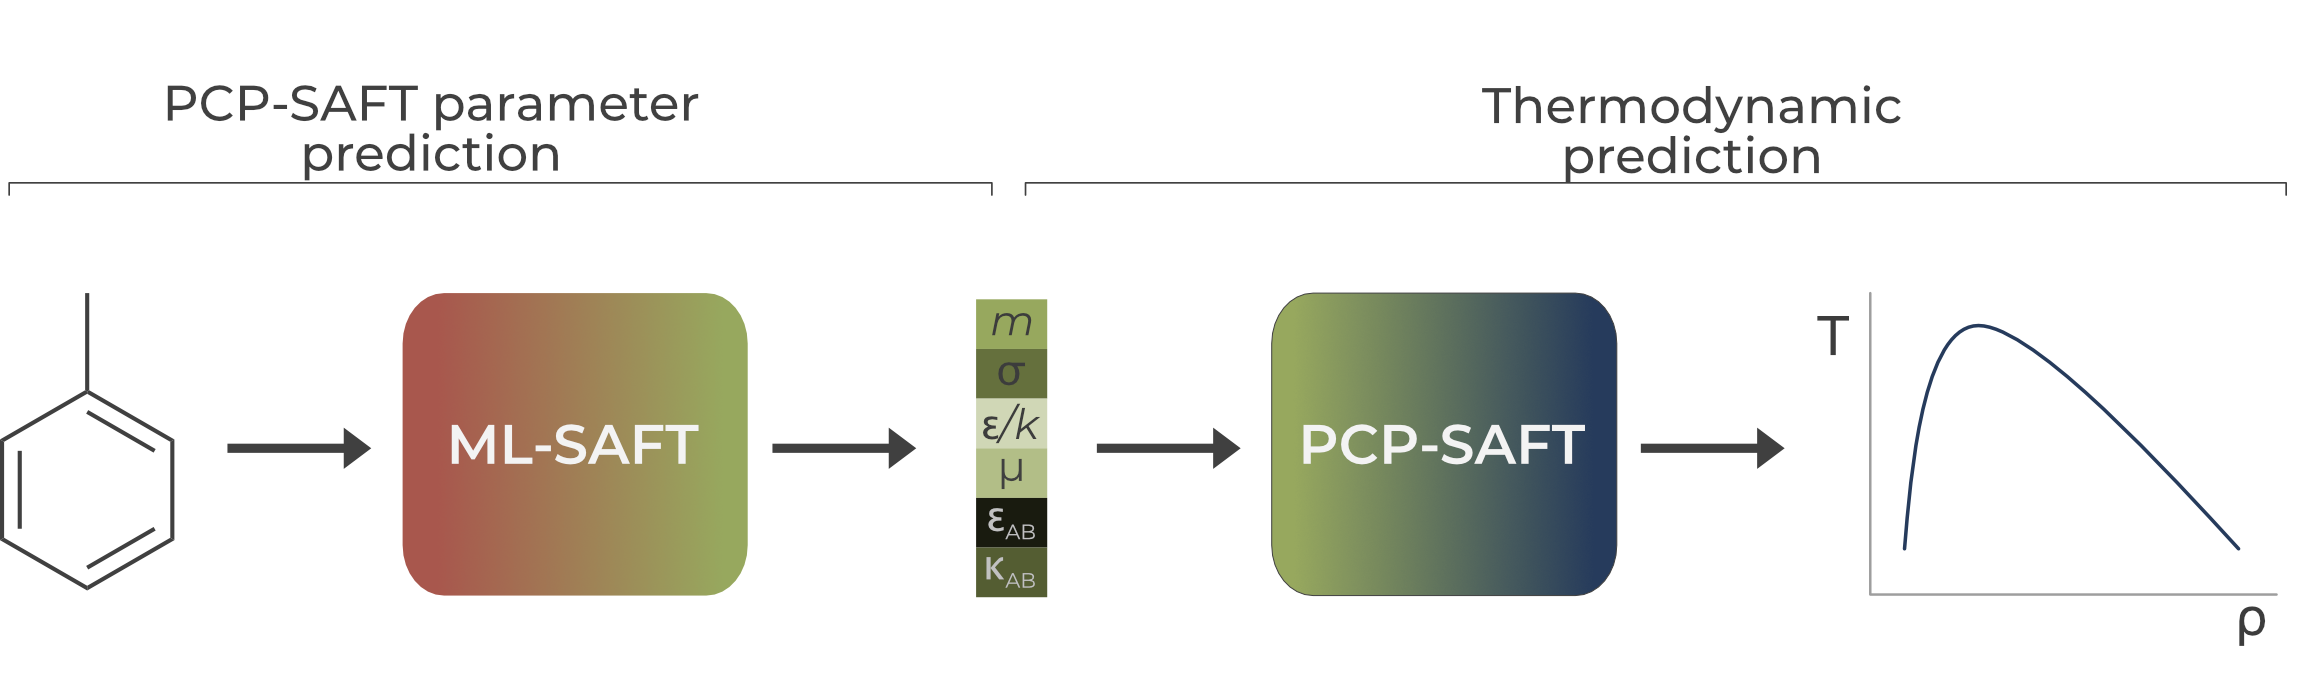
\includegraphics[width=\textwidth]{gfx/Chapter08/mlsaft_workflow.png}
    \caption{ML-SAFT is a framework for predicting PCP-SAFT parameters directly from molecular structures. PCP-SAFT parameters predicted by ML-SAFT models can be used in any PCP-SAFT implementation. Shown schematically is a density prediction.}
    \label{fig:ML-SAFT_workflow}
\end{figure}

I note that Habicht et al. \cite{Habicht2023} recently developed a feed forward neural network model to predict only PC-SAFT parameters from molecular fingerprints. The work presented in this chapter includes the polar and associating terms and a larger database of regressed PCP-SAFT parameters. I additionally found that random forests outperformed feedforward networks for PCP-SAFT parameter prediction.

\section{Methods}

\subsection{The PCP-SAFT equation of state}

In the formulation of PCP-SAFT \cite{Gross2001, Gross2006}, the Helmholtz free energy is calculated with respect to a reference a hard chain (hc) non-interacting fluid. Terms are added for dispersion (disp), association (assc) and dipole moments (dip):
\begin{equation}
    \frac{a}{kT} = \frac{a^{hc}}{kT} +  \frac{a^{disp}}{kT}  + \frac{a^{assc}}{kT} + \frac{a^{dip}}{kT}
    \label{eq:pcsaft_hemholtz}
\end{equation}

Each of these terms is calculated via equations derived from statistical mechanics. These equations in total have six pure component parameters for each molecule that must be regressed or predicted: $\sigma$, the hard sphere diameter; $m$, the number of segments in a chain of a component; $\epsilon/k$, the depth of the well; $\mu$, the dipole moment; and $\epsilon_{AB}$ and $\kappa_{AB}$, the association parameters. The goal of ML-SAFT is to predict these six pure component parameters directly from molecular structures. I use the implementation of PCP-SAFT in FeO$_{s}$ \cite{Rehner2023}.


% The Perturbed-chain statistical associating theory (PC-SAFT) EoSequation of state is derived in terms of the specific Hemholtz free energy \cite{Gross2001}. Given the Hemholtz free energy, other thermodynamic variables such as the pressure and fugacity coefficient can be derived. TIn the formulation of PC-SAFT, the Hemholtz free energy is calculated with respect to a   a reference a hard chain (hc) non-interacting fluid. Terms are added for dispersion (disp), association (assc) and dipole moments (dip):
% \begin{equation}
%     \frac{a}{kT} = \frac{a^{hc}}{kT} +  \frac{a^{disp}}{kT}  + \frac{a^{assc}}{kT} + \frac{a^{dip}}{kT}
%     \label{eq:pcsaft_hemholtz}
% \end{equation}
% For convenience, Equation \ref{eq:pcsaft_hemholtz} can be rewritten in terms of the compressibilty $Z=Pv/RT=a/kT$.
% \begin{equation}
%     Z = Z^{hc}+Z^{disp}+Z^{assc}+Z^{dip}
% \end{equation}

% PC-SAFT has four parameters that are regressed to experiments:  $\sigma$, the the cutoff soft repulsion in the hard chain;,$m$, number of segments in a chain of a component; $\epsilon/k$, the depth of the well; and $\mu$, the dipole moment. These are the four parameters that we predict in this paper, and in the following, we illustrate where each of these parameters is used in PC-SAFT EoS.

% To derive the hard chain term $Z^{hc}$, first define  a step function for the describe the pair potential energy:
% \begin{equation}
%     u(r) = \begin{cases} 
%         \infty & r < (\sigma - s_1) \\
%         3\epsilon & (\sigma - s_1) \leq r < \sigma \\
%         -\epsilon & \sigma \leq r < \lambda \sigma \\ 
%         0 & r\geq \lambda \sigma  
%     \end{cases}
% \end{equation}
% where $\epsilon$ is the depth of the well, $\sigma$ controls the cutoff for soft repulsion and $\lambda$ is the reduced well depth.  Therefore, the compressibility term for hard chain reference can be written as:
% \begin{equation}
%     Z^{hc} = \tilde m Z^{hs}- \sum_i x_i(m_i-1)\rho \frac{\partial \ln g_{ii}^{hs}}{\partial \rho}
% \end{equation}
% \begin{equation}
%     \tilde m = \sum_i x_i m_i
% \end{equation}
% where $m$ is the number of segments in a chain of component $i$ and $\rho$ is the number density of the molecules. $Z^{hs}$ is the hard-sphere compressibility and $g^{hs}$ is the radial distribution for segments in the hard sphere reference.  
% \begin{equation}
%     Z^{hs} = \frac{\xi_3}{1-\xi_3} + \frac{3\xi_1\xi_2}{\xi_0(1-\xi_3)^2} + \frac{3\xi^3-\xi_3\xi_2^3}{\xi_0(1-\xi_3)^3}
% \end{equation}
% \begin{equation}
%     g_{ij}^{hs} = \frac{1}{1-\xi_3} + \biggl(\frac{d_id_j}{d_i + d_j}\biggr)\frac{3\xi_2}{1-\xi_3}+\biggl(\frac{d_id_j}{d_i + d_j}\biggr)^2\frac{2\xi_2^2}{(1-\xi_3)^3}
% \end{equation}
% \begin{equation}
%     \xi_n = \frac{\pi}{6} \rho \sum_i x_im_i d_i^n \;\; n\in \{ 0, 1, 2, 3,\}
% \end{equation}
% \begin{equation}
%     d(T) = \int_0^{\sigma} \biggl[1 - \exp \biggl(-\frac{u(r)}{kT} \biggr)\biggr]dr
% \end{equation}
% To derive the pertubation due dispersion $Z^{disp}$, a second order Hemholtz formulation is used:
% \begin{equation}
%     \frac{a^{disp}}{kTN} = \frac{a_1}{kT} +  \frac{a_2}{kT}
% \end{equation}
% \begin{equation}
%     {Z^{disp} = Z_1 + Z_2}
% \end{equation}
% The two terms are derived using results from Gross and Sadowski.\cite{Gross2001}

% To derive the associative term $Z^{assc}$...

% To derive the polar term $Z^{dip}$,


% has strong performance for predicting fluid-phase equilibria of a variety of mixtures. Four parameters need to be predicted for any pure component and 2 extra parameters for mixtures. If we can predict parameters, EoS ensures thermodynamic consistency.


\subsection{Baseline predictive PCP-SAFT methods}\label{sec:baselines}

There are several methods in the literature for predicting PCP-SAFT parameters. As comparisons to ML-SAFT, I evaluated two state-of-the-art methods that use QM and a group contribution method respectively.

As a QM method, the Segment-Based Equation of State Parameter Prediction (SEPP) was applied \cite{Kaminski2020}. All SEPP calculations were carried out by Lukas Ra{\ss}pe-Lange. SEPP obtains $m$, $\sigma$, and $\epsilon/k$ from a multilinear model that uses DFT-calculated features as input, while the dipole moment $\mu$ is obtained directly from QM calculations. An analysis of the surface charge density from COSMO was utilized to calculate the associating parameters $\epsilon_{AB}$ and $\kappa_{AB}$ \cite{Klamt1995}. The strongest associating site was used although SEPP can take into account all binary associating interactions. This simplification was made to ensure that the predicted parameters could be used with most PCP-SAFT implementations. Since the multilinear model in SEPP was only fit to alkanes and polar compounds with oxygen and nitrogen, it is not valid for halogens, which are abundant in my dataset.

I used the homosegmented group contribution method from Sauer et al \cite{Sauer2014} as implemented in FeO$_{s}$ \cite{Rehner2023}. We used the fitted parameters from Sauer et al for all predictions. Some molecules in our dataset were not already segmented into groups by Sauer et al, so we used an algorithm from the python package thermo \cite{thermopython} to identify the groups that should be used for prediction.  A modified version of the SMARTS strings from Ruggeri and Takahama (see Supplementary Material) were used in the algorithm \cite{Ruggeri2016}.

\subsection{Building a dataset for ML-SAFT}\label{subsec:data_set}

% To provide data for training ML models, I built, to my knowledge, the largest dataset of PCP-SAFT parameters available to date in the literature (988 molecules).

\subsubsection{Data extraction from the Dortmund Data Bank}

Experimental data were extracted from the 2022 Dortmund Data Bank, which contains data for over 40k unique molecules \cite{dortmunddatabank}. The software package Pura \cite{purapython} was used to resolve the name or CAS numbers available in the Dortmund database into a cheminformatics friendly identifier, namely SMILES. Pura called on PubChem \cite{Kim2020}, the Chemical Identifier Resolver \cite{cir}, OPSIN \cite{Lowe2011}, and the Chemical Abstracts Service \cite{commonchem} to resolve a name or CAS number, and I required that at least two services agreed on the resolved SMILES. Pura resolved 68\% (27.2k/40.3k) of names or CAS numbers to SMILES. 

The experimental data were subsequently filtered to obtain only data that were reasonable for PCP-SAFT regression. Ionic molecules were removed from the dataset as well as any molecules with temperatures outside of the range 200-1000 K and pressures outside the range 10-10000 kPa. Densities greater than 2000 $\text{kg/m}^{3}$ were also excluded. Finally, only molecules with at least four density data points and five vapor pressure data points were considered. After all filtering steps, the experimental data for 988 unique molecules were available for regression of PCP-SAFT parameters. This significant decrease in the size of the data set from 27k to 1k by the filtering step has been noted in other attempts to build models using data available in literature databases \cite{Fitzner2020, Gao2018}. 

\subsubsection{PCP-SAFT parameter regression}

To find optimal PCP-SAFT parameters for each compounds, I used the well-established Levenberg-Marquardt (LM) least squares algorithm and experimental vapor pressure and density data, as shown in Figure \ref{fig:ML-SAFT_regression}. The same initial guess shown in Table \ref{tab:regression_params} was applied for all molecules, which was based on the analysis of a large set of PCP-SAFT parameters calculated by QM simulation (see Section \ref{sec:baselines}) \cite{Kaminski2020}. The following equation was applied to calculate the sum of squared errors $\mathcal{L}_i$ for molecule $i$:
\begin{gather}
\begin{aligned}
    \mathcal{L}_i & = \; \sum_j \biggl(\frac{p_{i}^{sat,\text{SAFT}}(T_j) - p_{i}^{sat,\text{EXP}}(T_j)}{ p_{i}^{sat,\text{EXP}}(T_j)}\biggr)^2 \\
    & \; + \sum_j \biggl(\frac{\rho_{i}^{l,\text{SAFT}}(T_j, P_j) - \rho_{i}^{l,\text{EXP}}(T_j, P_j) }{\rho_{i}^{l,\text{EXP}}(T_j, P_j) }\biggr)^2 
\end{aligned}
\end{gather}
where $p_i^{sat}(T_j)$ and $\rho_{i}^{l}(T_j, P_j)$ are the saturation vapor pressure and the liquid density for molecule $i$ respectively at temperature $T_j$ and $P_j$. The superscripts $\text{SAFT}$ and $\text{EXP}$ represent PCP-SAFT predictions and experimental data respectively. 

\begin{table}
    \centering
    \caption{Parameters fitted in PCP-SAFT regression to experimental data.}
    \label{tab:regression_params}
    \begin{tabular}{ccc}
        Parameter name & Bounds & Initial Value \\
        \hline
        $m$ & $1.0 \leq m \leq 10.0$ & 3.26 \\
        $\sigma$ & $2.5 \leq \sigma \leq 5.0$ & 3.69 \\
        $\epsilon/k$ & $100.0 \leq \epsilon/k \leq 1000.0$ & 284 \\
        % $\mu$ & $0.0 \leq \mu \leq 10.0$ & $mu_{pred}$ \\
        $\epsilon_{AB}$ & $0.0 \leq \epsilon_{AB} \leq 4000.0$ & 2400 \\
        $\kappa_{AB}$ & $0.0 \leq \kappa_{AB} \leq 0.01$ & 0.0 \\
        \hline
    \end{tabular}
\end{table}


\begin{figure}
    \centering
    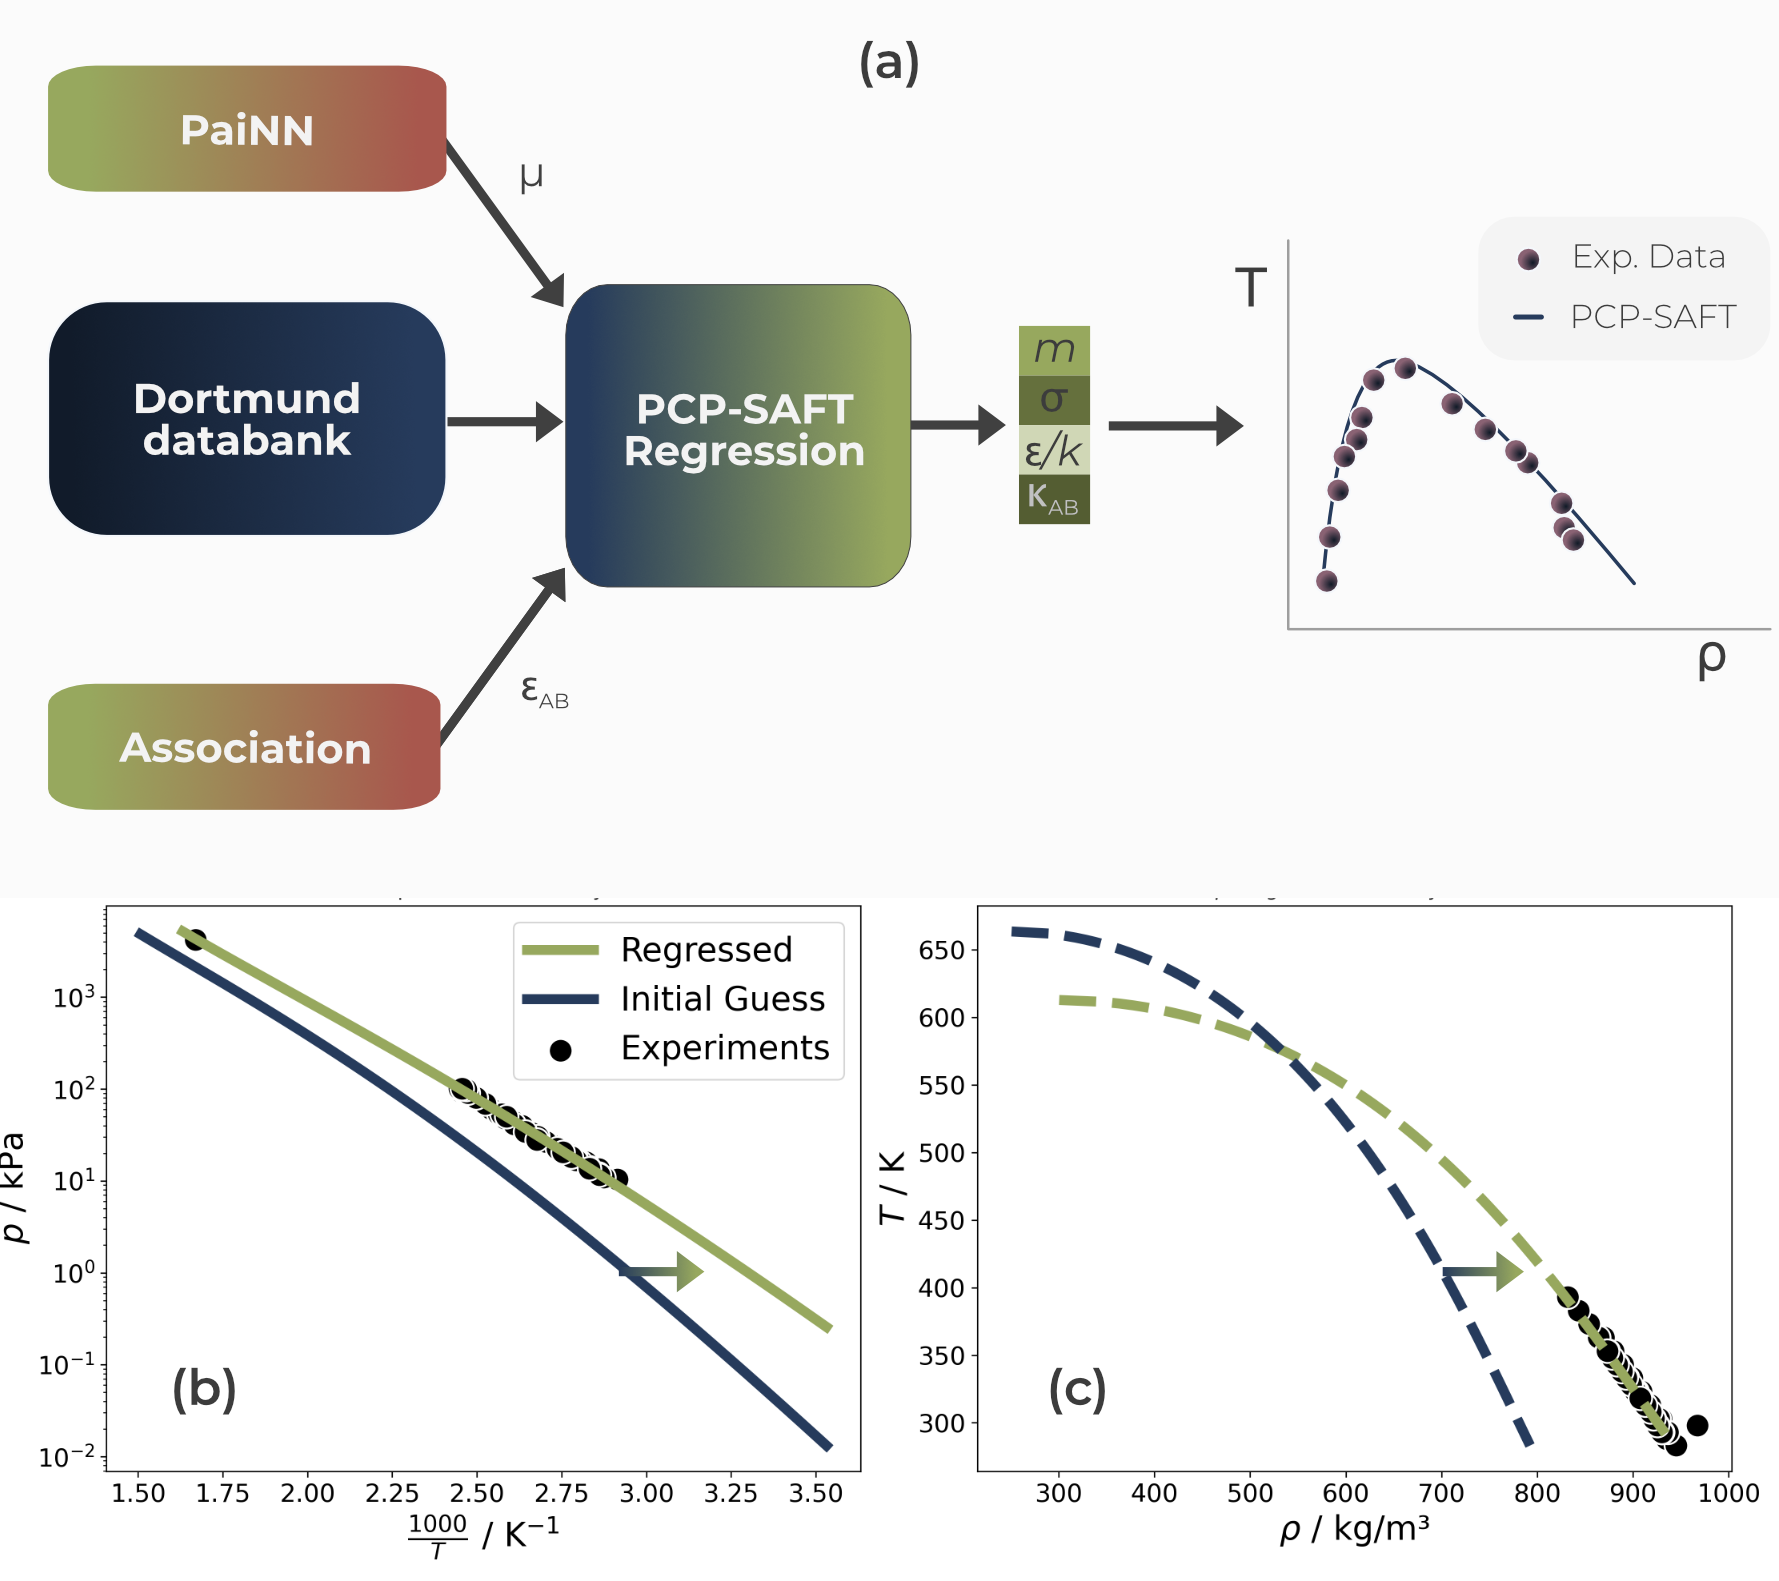
\includegraphics[width=\textwidth]{gfx/Chapter08/deepsaft_regression.png}
    \caption{Building a dataset for ML-SAFT: (a) A workflow was developed to automatically regress PCP-SAFT parameters to pure component experimental data. A machine learning model (PaiNN) trained on  a combination of DFT and experimental data were used to predict the dipole moments of the experimental dataset, and the other parameters were initialized using standard values. (b-c) Example regression of PCP-SAFT to vapor pressure and density data for 2-ethoxyethanol using the Levenberg-Marquandt algorithm. Experiments are data from the Dortmund Databank \cite{dortmunddatabank}. The dashed line in the density plot represents liquid density.}
    \label{fig:ML-SAFT_regression}
\end{figure}

Only $m$, $\sigma$, $\epsilon/k$ were regressed for all molecules, and $\epsilon_{AB}$ was additionally regressed for associating molecules, while $\mu$ and $\kappa_{AB}$ were not regressed. The dipole moment $\mu$ was predicted and used heuristics to determine if a molecule was associating (described below). The choice to predict the dipole moment is justified for two reasons. First, the dipole moment can usually be measured or calculated on a physical basis, and second, previous work has shown that adjusting the dipole moment causes regression to fail due to high correlation with $\epsilon/k$ \cite{Cripwell2017, deVilliers2011}. 

Therefore, I trained a deep learning model to predict dipole moments using a combination of DFT calculated and experimentally determined dipole moments, as shown in Table \ref{tab:painn_data}.  Once trained, the model made dipole moment predictions for hundreds of molecules in seconds. For the model architecture, I chose the tensorial equivariant message passing neural network PaiNN developed by Schütt et al. since it has been shown to give accurate predictions of dipole moment \cite{Schutt2021}. Note that the initial implementation of this model was completed by Jan Rittig. Briefly, PaiNN takes as input a relaxed conformer of a molecule and uses a series of message passing steps on both a vector and rank three tensorial representation to produce a representation of each atom. For training, I used the conformer generation methods shown in Table \ref{tab:painn_data}, and for inference, I used the RDKit ETKDGv3 algorithm to generate conformers \cite{Wang2020}. Subsequently, the dipole moment was calculated using the final vector and tensorial representations of the network:

\begin{equation}
    \vec \mu = \biggl [\sum_{i=1}^N \vec \mu_{atom}(\vec{\mathbf v_i}) + q_{atom}(\mathbf s_i)\vec r_i \biggr ]
\end{equation}
where $\mathbf s_i$ is the vector representation and $\mathbf v_i$ is the tensorial representation, $\vec r_i$ are the positions of the atoms and $\mu_{atom}$ and $q_{atom}$ are both feedforward networks. Training for 63 epochs resulted in a validation mean absolute error of 0.005 for held-out dipole moment predictions.

We created two heuristics for improving regression of association parameters. First, non-associating molecules were defined as molecules not containing at least one hydrogen-bond acceptor and donor site via RDKit \cite{rdkit}. The associating parameters $\epsilon_{AB}$ and $\kappa_{AB}$ were set to zero for these non-associating molecules. Second, I found that associating parameter $\kappa_{AB}$ could be set to 0.01 and not regressed for all associating molecules while maintaining low regression error. With the deep learning predictions of $\mu$ and the heuristics for association in place, I successfully regressed PCP-SAFT parameters for the 988 available molecules. 

\begin{table}[]
    \centering
    \caption{Data sets used to train PaiNN architecture for predicting dipole moments. $\mu_{source}$ is method used to generate dipole moments; DFT is density functional theory, and Exp. is experimental.}
    \begin{tabular}{ccccc}
         Dataset & $\mu_{source}$ & Conformer Type & Size & Ref.  \\
         \hline
         QM9 & DFT & DFT & 134k & \cite{Ramakrishnan2014}\\
         CRC & Exp. & RDKit\cite{Wang2020} & 482 & \cite{CRC2014} \\
         SEPP & DFT & DFT & 1106 & See Section \ref{sec:baselines} \\
         \hline
    \end{tabular}

    \label{tab:painn_data}
\end{table}

\subsubsection{COSMO-RS data generation}

In addition to the Dortmund data bank dataset, I generated a set of PCP-SAFT parameters utilizing pseudo experimental data from the fluid-phase thermodynamics program COSMO-RS \cite{Klamt2010}. Specifically, I generated vapor pressure and density data for 3488 molecules that were already in available 2020 version of the COSMO-RS database. I then regressed PCP-SAFT parameters to these COSMO-RS datasets using the same methods described above. This resulted in 2680 parameters sets available for training.

\subsection{ML-SAFT machine learning models}\label{subsec:ML-SAFT_model}

For prediction of the regressed PCP-SAFT parameters from molecular structures, I tested several machine learning architectures that have previously been successfully applied to molecular property prediction tasks. I included a random forest (RF) \cite{Breiman2001} and a standard feed-forward network (FFN) that use ECFP4 fingerprints with 2048 bits as input features \cite{Rogers2010}. RFs are known to have strong performance for molecular property prediction in drug discovery but are less common in chemical engineering \cite{Ramsundar2017, Yang2019}. Feed-forward networks were used successfully by Habicht et al. in previous work on predicting PCP-SAFT parameters \cite{Habicht2023}. Furthermore, I developed a standard message passing neural network (MPNN) \cite{Gilmer2017} that has previously been used to predict several thermodynamic parameters including fuel properties \cite{Schweidtmann2020} and activity coefficients \cite{SanchezMedina2022, Rittig2023}. MPNNs construct a graph representation where atoms are represented as nodes and bonds as edges. By iteratively passing information contained in features between the nodes, the model builds up atom features, which are averaged to create a fixed length learned feature vector that can be passed through a feed-forward network. I also tested a variant of an MPNN in which the encoder acts on edges (bonds) instead of nodes (atoms); this architecture is called a directed MPNN (D-MPNN) and has been shown to have state-of-the-art performance for molecular property prediction \cite{Yang2019, Vermeire2021}. Table \ref{tab:model_features} summarizes the input features used for each model.  

All neural network models (FFN, MPNN and D-MPNN) were trained in multi-task mode to predict all parameters simultaneously for 1000 epochs to minimize the mean squared error loss between the predicted and regressed PCP-SAFT parameters using the Adam optimization algorithm \cite{Kingma2015} and the Noam scheduler \cite{Vaswani2017}. The best model checkpoint according to validation loss was used. The learning rate was tuned for each model. I found that using dropout after the pooling step in the MPNN and D-MPNN improved generalization performance. The hyperparameters for each model were explored using a quasi-random design with a budget of 100 trials \cite{Bosquet2017}. The best hyperparameters for each model architecture were selected by evaluating the sum of the RMSE for all PCP-SAFT parameters. All the final hyperparameters can be found in Table \ref{tab:hyperparameters}.

\begin{table}[t]
    \centering
    \caption{Input features for each model included in ML-SAFT}
    \begin{tabular}{cc}
         Model & Input Feature Transform \\
         \hline
         RF & SMILES $\rightarrow$ ECFP4 FPs \\
         FFFN & SMILES $\rightarrow$  ECFP4 FPs \\
         MPNN & SMILES $\rightarrow$  graph (nodes: atoms, edges: bonds) \\
         D-MPNN & SMILES $\rightarrow$  graph (nodes: bonds, edges: atoms) \\
    \end{tabular}
    \label{tab:model_features}
\end{table}

I experimented with two adaptations of ML to PCP-SAFT prediction. First, since I could already distinguish between associating and non-associating molecules using the heuristic from the regression step (i.e., checking the number of association sites), I automatically clamped the association parameters $\epsilon_{AB}$ and $\kappa_{AB}$ to zero for non-associating compounds. I evaluated this clamping of non-associating molecules both as a post-processing step for all models and, for the neural networks, inside the loss function of the neural network. Second, I observed that there were more non-associating than associating molecules in the dataset. Therefore, I tested oversampling of associating molecules in each batch during neural network training using a weighted random sampler:
\begin{equation}
    w_i^{A} = \frac{1}{n_A}
\end{equation}
where $w_i^{A}$ is weight for molecule $i$ with association status $A$ and $n_A$ is the number of molecules of that association status in the whole dataset. I call this oversampling procedure balanced association sampling.

\subsection{Pretraining of MPNNs}

I also explored using pretraining to improve the quality of predictions from PCP-SAFT. Specifically, I pretrained the MPNN architecture on the PCP-SAFT parameters regressed to COSMO-RS data. Then, I froze the message passing encoder and only trained the feed forward portion of the MPNN on the regressed parameters from Dortmund. I refer to this strategy as MPNN-TL.

\subsection{Evaluation of predictive PCP-SAFT methods}

To evaluate ML-SAFT models and the baseline predictive PCP-SAFT methods, a set of 81 molecules was held out from training any models and only used for testing. These molecules were selected as the (1) intersection of molecules that could be predicted by SEPP and the group contribution method; and (2) a set of halides since SEPP did not work this class of molecules. I then split the remaining 905 molecules into training and validation (5 \%) sets using a clustering procedure. Specifically, ECFP fingerprints with 2048 bits were generated using RDKit, and the k-means clustering algorithm \cite{MacQueen1967} was run on five dimensional projections of these fingerprints from the dimensionality reduction tool UMAP \cite{McInnes2018}. I found three clusters to most effectively model the data, as shown in Figure \ref{fig:splitting}a. Upon manual inspection, I found that the clusters represented chemically interpretable classes of molecules such as alkanes and aromatics. Finally, the molecules were assigned to the training and validation sets so that cluster proportions in each split matched the cluster proportions in the overall dataset using the Stratified Shuffle Split method in scikit-learn \cite{scikit-learn}. As shown in Figure \ref{fig:splitting}c, this ensured that each split in the training and validation set had a balanced set of molecules. Note that the test set had a different distribution due to the limitations of the baseline methods used for comparison.

\begin{figure}
    \centering
    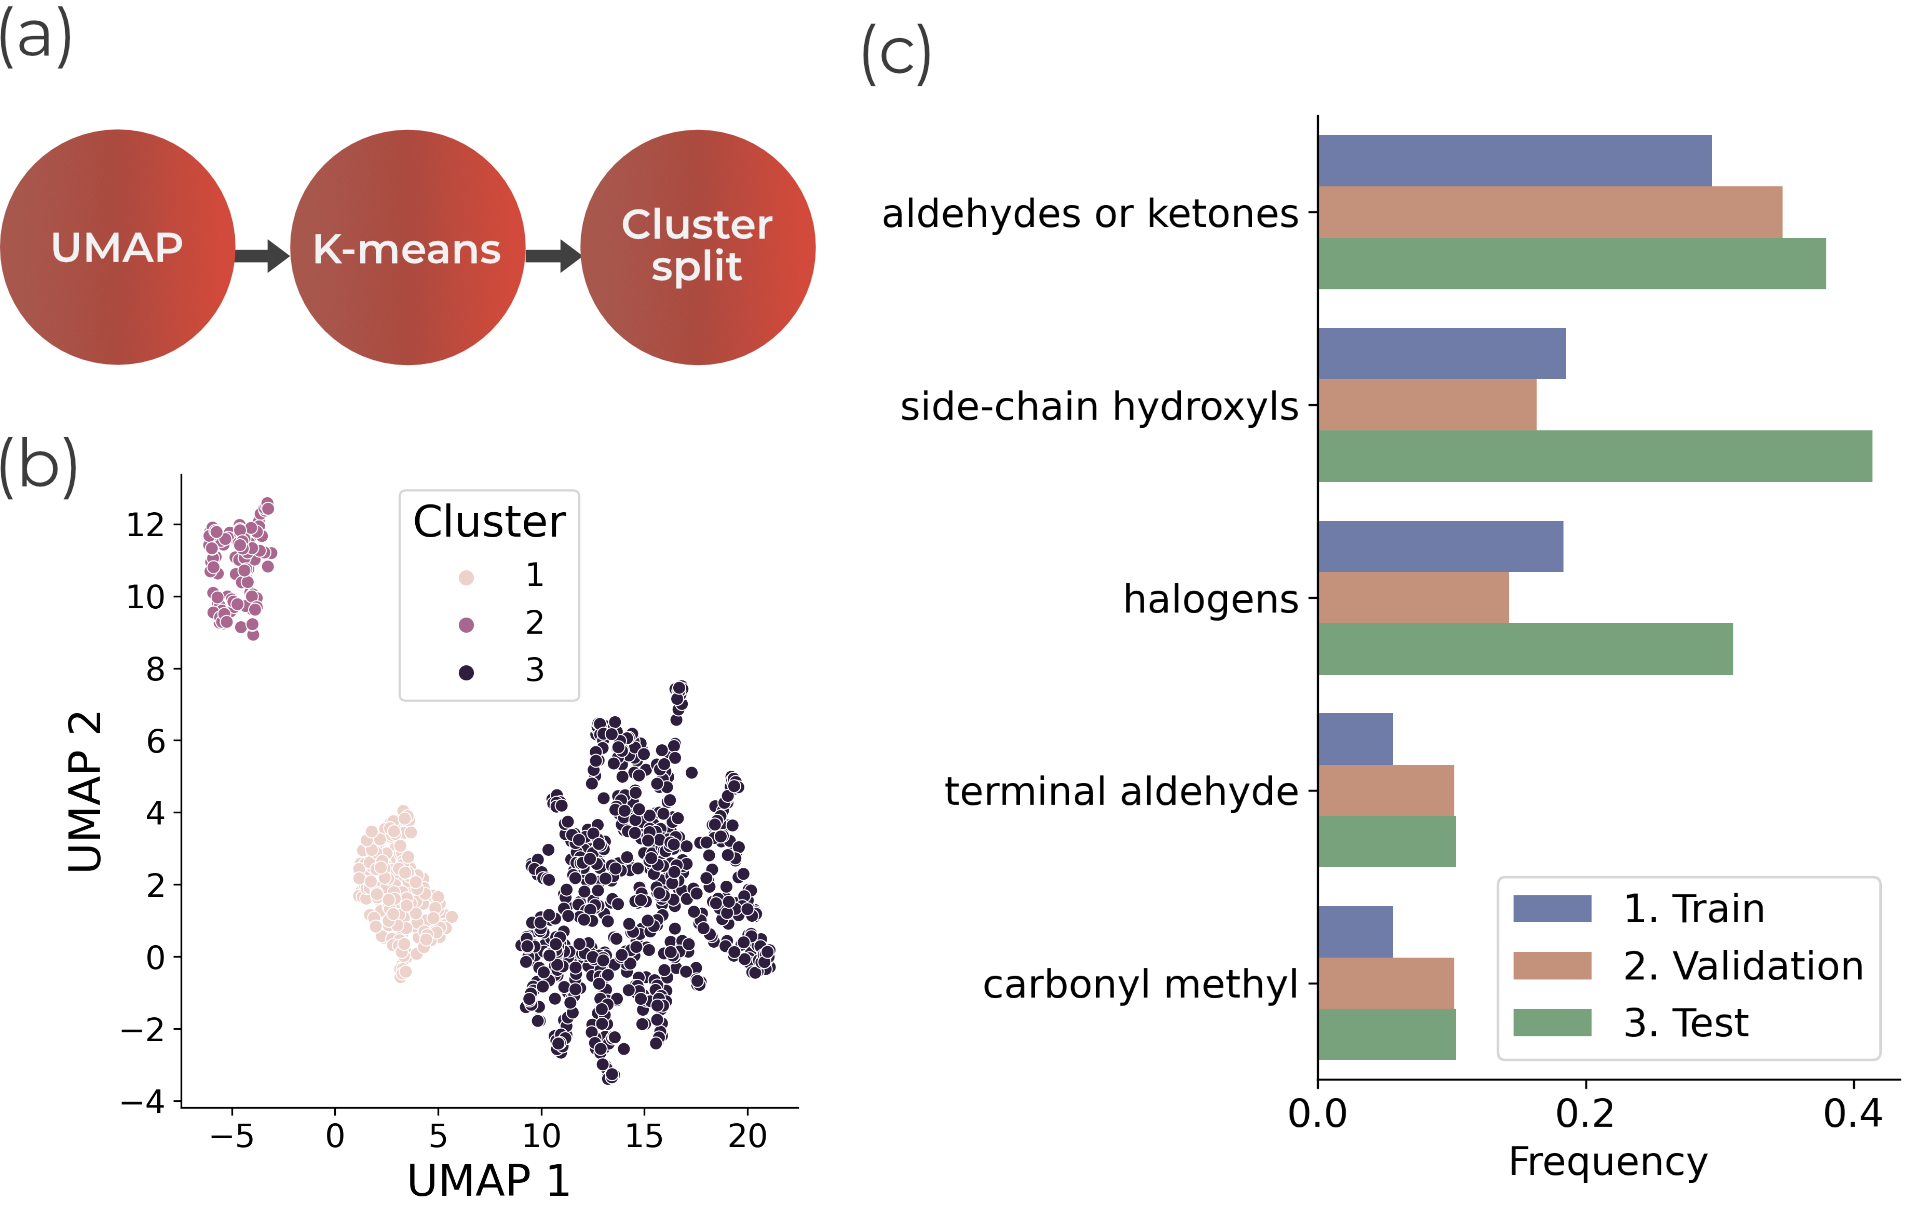
\includegraphics[width=\textwidth]{gfx/Chapter08/cluster_split.png}
    \caption{Data splitting for ML-SAFT datasets. (a) Schematic of the workflow for stratified splitting of the ML-SAFT dataset. UMAP \cite{McInnes2018} is used for dimensionality reduction of 2048 bit ECFP fingerprints followed by k-means clustering \cite{MacQueen1967} and cluster splitting using stratified shuffle split in scikit-learn \cite{scikit-learn}. (b) 2D visualization of the clustering using UMAP. (c) The frequency of the top five functional groups in each split are shown.}
    \label{fig:splitting}
\end{figure}

I used two metrics for evaluation of the models. For the evaluation of the error between the parameter predictions and regressed parameters, I applied the root mean squared error (RMSE):
\begin{equation}
    \text{RMSE} = \sqrt{\sum_{i=1}^N \frac{(y_i - \hat y_i)^2}{N}}
\end{equation}
where $y_i$ is the regressed PCP-SAFT parameter and $\hat y_i$ is the predicted PCP-SAFT parameter. For evaluation of the predictions of density and vapor pressure, I used the percent absolute average deviation (\% AAD):
\begin{equation}
    \% AAD = 100 \biggl \vert \sum_j\frac{Q_J - \hat Q_j}{Q_j} \biggr \vert  
\end{equation}
where $Q$ is the experimental value of vapor pressure or liquid density and $\hat Q$ is the corresponding PC-SAFT prediction.

\section{Results}

\subsection{A robust regression method for PCP-SAFT parameters}

We sought to develop an automated approach to regressing the PCP-SAFT parameters from experimental data. Since we used the same initial guess for the regression of all 988 molecules in our dataset, we first aimed to understand the quality of this initial guess across the dataset. As shown in Figure \ref{fig:regression_errors}(a-b), the standard initial guess gave liquid density initialization with 37 \%AAD on average, while the initial accuracy for vapor pressure predictions were significantly worse with an average of 380 \%AAD. The larger errors for vapor pressure are likely due to the values for vapor pressure varying over several orders of magnitude. However, after regression, most of the PCP-SAFT predictions had less than 5 \%AAD, and the overall average was 3.84 \%AAD for vapor pressure predictions and 0.79 \%AAD for liquid density predictions, as shown in Figure \ref{fig:regression_errors}(c-d). Empirically, we found that the most important factor for successful regression was the choice of parameter constraints, which we obtained using the maximum and minimum values from all SEPP calculations.

\begin{figure}
    \centering
    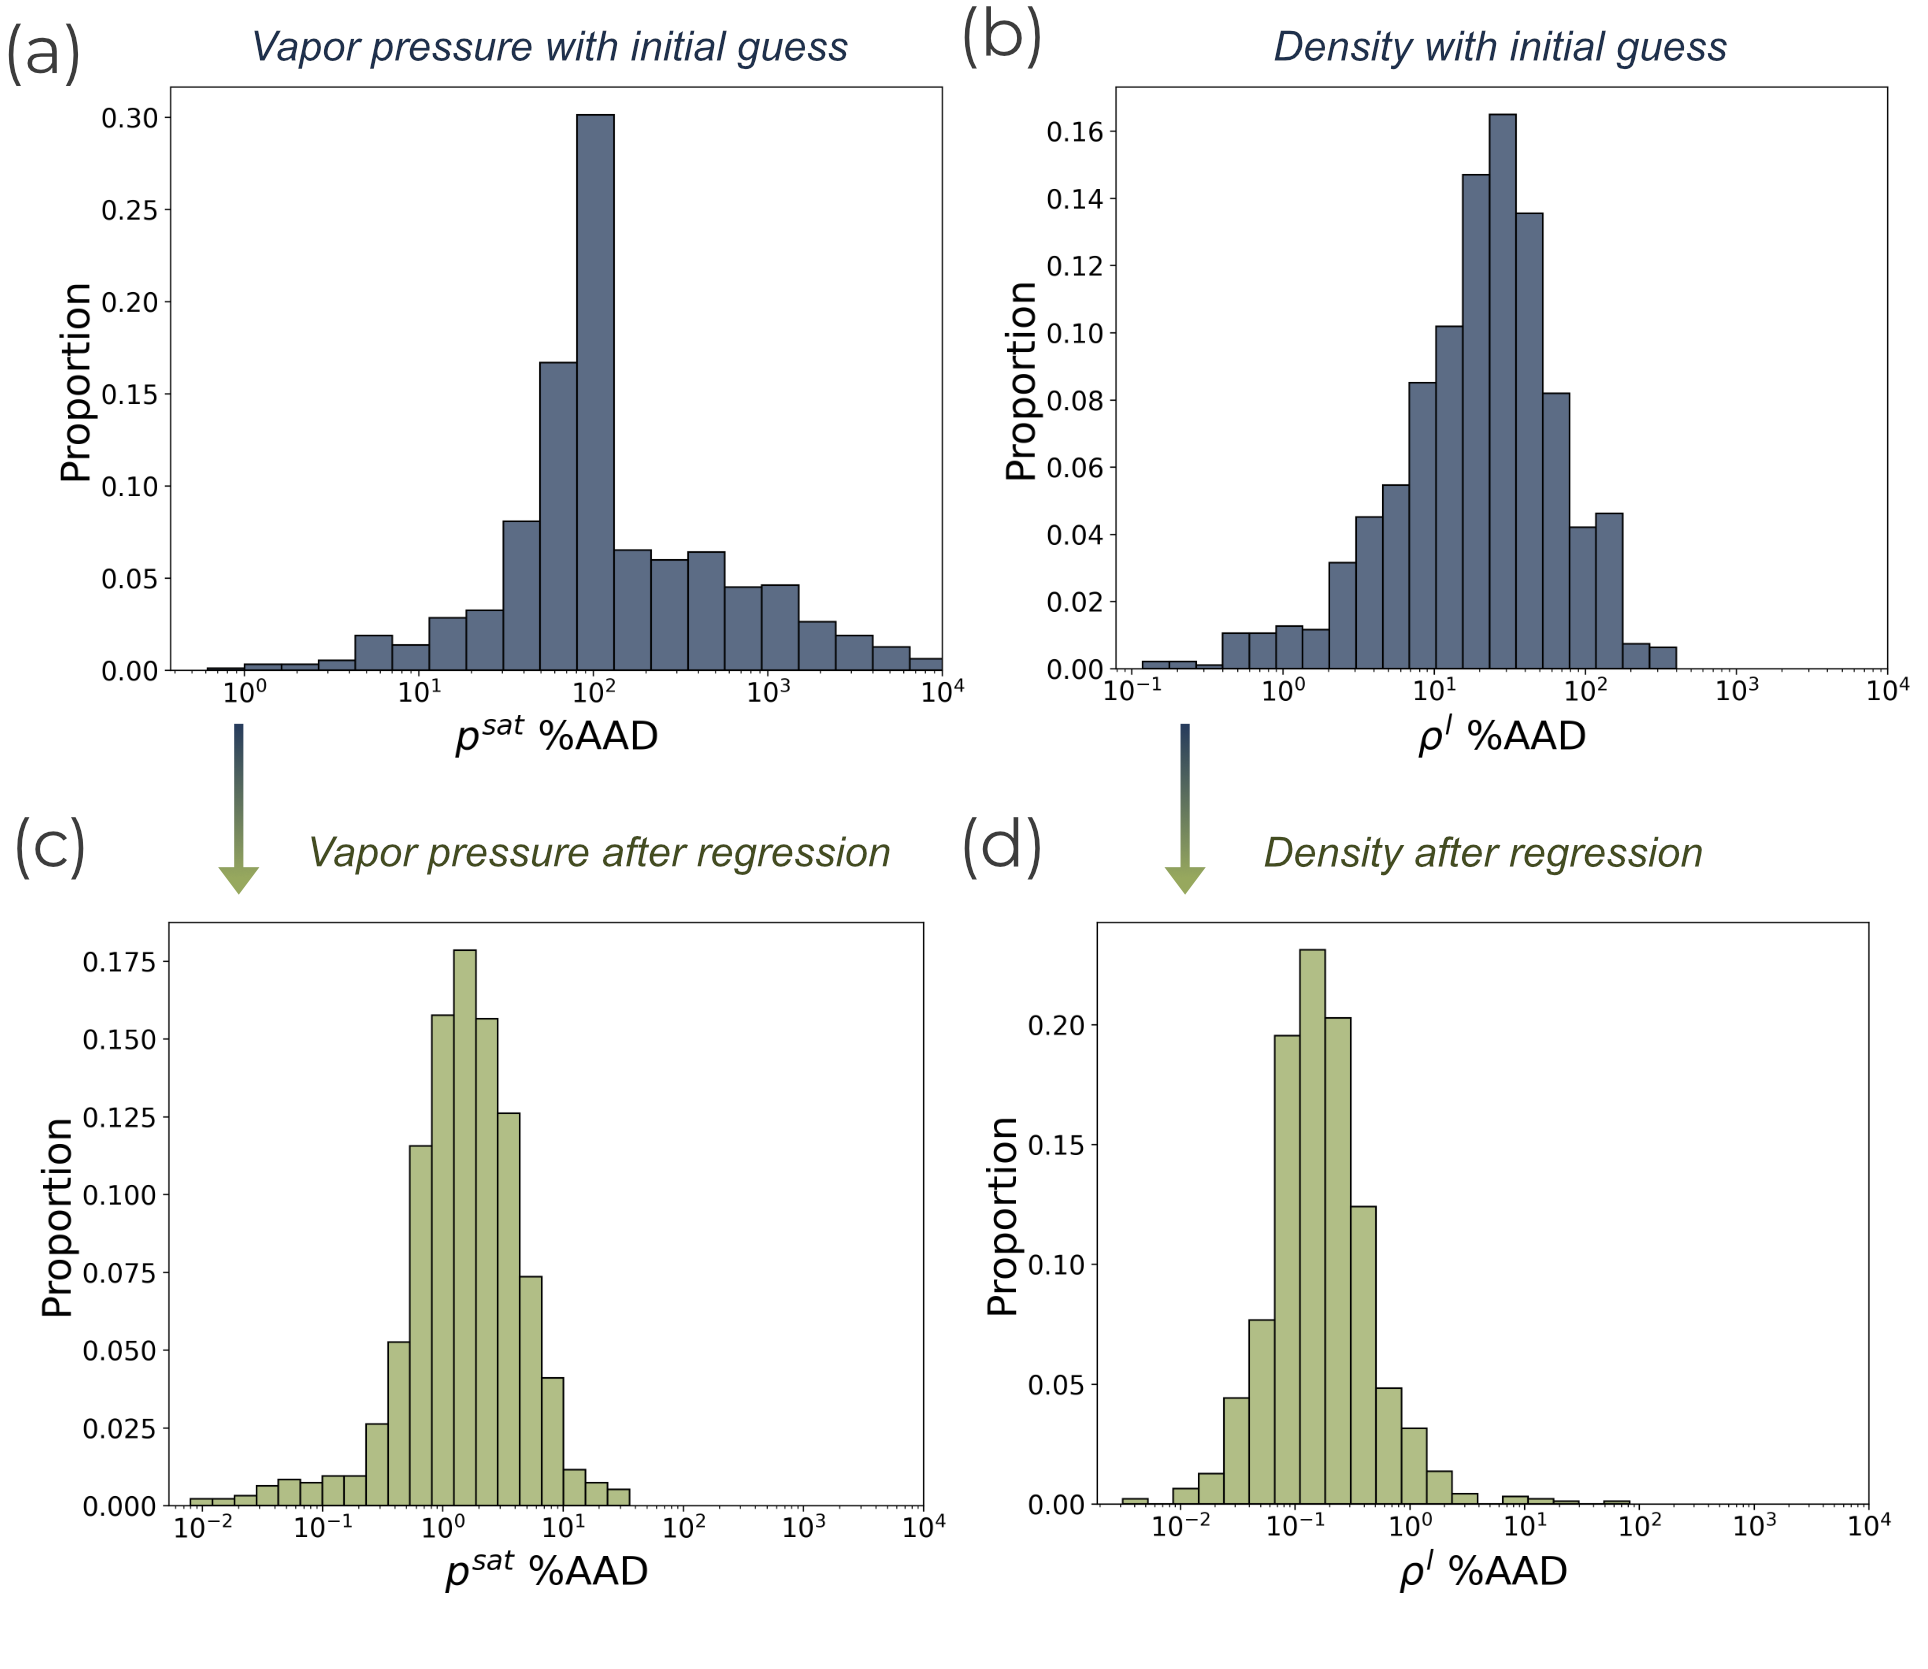
\includegraphics[width=\textwidth]{gfx/Chapter08/regression_errors.png}
    \caption{Distribution of \%AAD  when using PCP-SAFT regressed parameters for all molecules in the ML-SAFT dataset. (a) Initial guess vapor pressure (b) Initial guess liquid density (c) Regressed vapor pressure (d) Regressed liquid density.}
    \label{fig:regression_errors}
\end{figure}

\subsection{ML-SAFT accurately predicts regressed PCP-SAFT parameters}

To evaluate the accuracy of ML models trained to predict the regressed PCP-SAFT parameters, I first compared the PCP-SAFT parameter predictions from the ML models with the regressed PCP-SAFT parameters. Table \ref{tab:parameter_predictions} shows the RMSE of PCP-SAFT parameter predictions from the various machine learning architectures (full parity plots are shown in the \ref{app:parity}). The RF with ECFP fingerprints performed best in predicting PCP-SAFT parameters. Even after hyperparameter tuning, all neural network architectures had up to 200\% worse RMSE values. Compared to previous work by Habicht who found that feed forward neural networks gave accurate predictions, my dataset provides a more difficult regression task as I consider a wider range of molecules and predict polar parameters for associating molecules; this might explain the lower accuracy of the feed forward neural networks in this case. However, the accuracy of predictions of regressed PCP-SAFT parameters might not always translate to the accuracy of thermodynamic predictions, so I also sought to compare the quality of vapor pressure and density predictions.

\begin{table}
	\caption{RMSE (lower is better) of each model architecture.  The best score for each target is marked in bold. RF: Random forest, FFN: Feed-forward neural network, MPNN: Message-passing neural network, D-MPNN: Directed message-passing neural network.}
        \label{tab:parameter_predictions}
	\begin{center}
        \begin{tabular}{lrrrr}
        	 & FFN & D-MPNN & MPNN & RF \\
        	\hline
        	$m$ & 0.59 & 0.85 & 0.98 & \textbf{0.54} \\
        	$\sigma$ & 0.28 & 0.34 & 0.35 & \textbf{0.26} \\
        	$\epsilon/k$ & 39.3 & 39.3 & 42.7 & \textbf{31.3} \\
        	$\epsilon_{AB}$ & 362 & 476 & 478 & \textbf{215} \\
                \hline
        \end{tabular}
	\end{center}
\end{table}

Table \ref{tab:thermo_parameters} presents the absolute average deviation from experimental data of PCP-SAFT predictions of vapor pressure and liquid density using the predicted PCP-SAFT parameters from various ML models. The RF model gave the most accurate predictions for both the vapor pressure and the liquid density with an average of 39\% and 9\% AAD, respectively, for the molecules in the test set.

\begin{table}
	\caption{Comparison of thermodynamic predictions using PCP-SAFT parameters predicted by ML-SAFT models only. The best score for each thermodynamic quantity is marked in bold. $n$ is the number of molecules in the test set that each method can
predict.}
	\begin{center}
        \label{tab:thermo_parameters}
        \begin{tabular}{lrrrr|r}
        	 & FFN & D-MPNN & MPNN & RF & Regressed \\
        	\hline
        	$n$ & 81 & 81 & 81 & 81 & 81 \\
        	\%AAD $p_{sat}$ & 354 & 53.0 & 69.7 & \textbf{38.6} & 4.47 \\
        	\%AAD $\rho^{L}$ & 11.3 & 9.76 & 13.9 & \textbf{8.64} & 0.800 \\
                \hline
        \end{tabular}
	\end{center}
\end{table}

I also experimented with several methods to adapt neural network training to PCP-SAFT parameter prediction. I found that there was no significant difference between clamping the values of the association parameters to zero as a post-processing step versus during training. Furthermore, balanced association sampling did not offer any noticeable improvement in the accuracy of PCP-SAFT parameter predictions. Although balanced association sampling improved predictions of the association parameter $\epsilon_{AB}$, it degraded the prediction accuracy of the other PCP-SAFT parameters and ultimately led to worse performance on the thermodynamic predictions. Full results of hyperparameter tuning can be found in Table \ref{tab:hyperparameters}.

% \begin{figure}
%     \centering
%     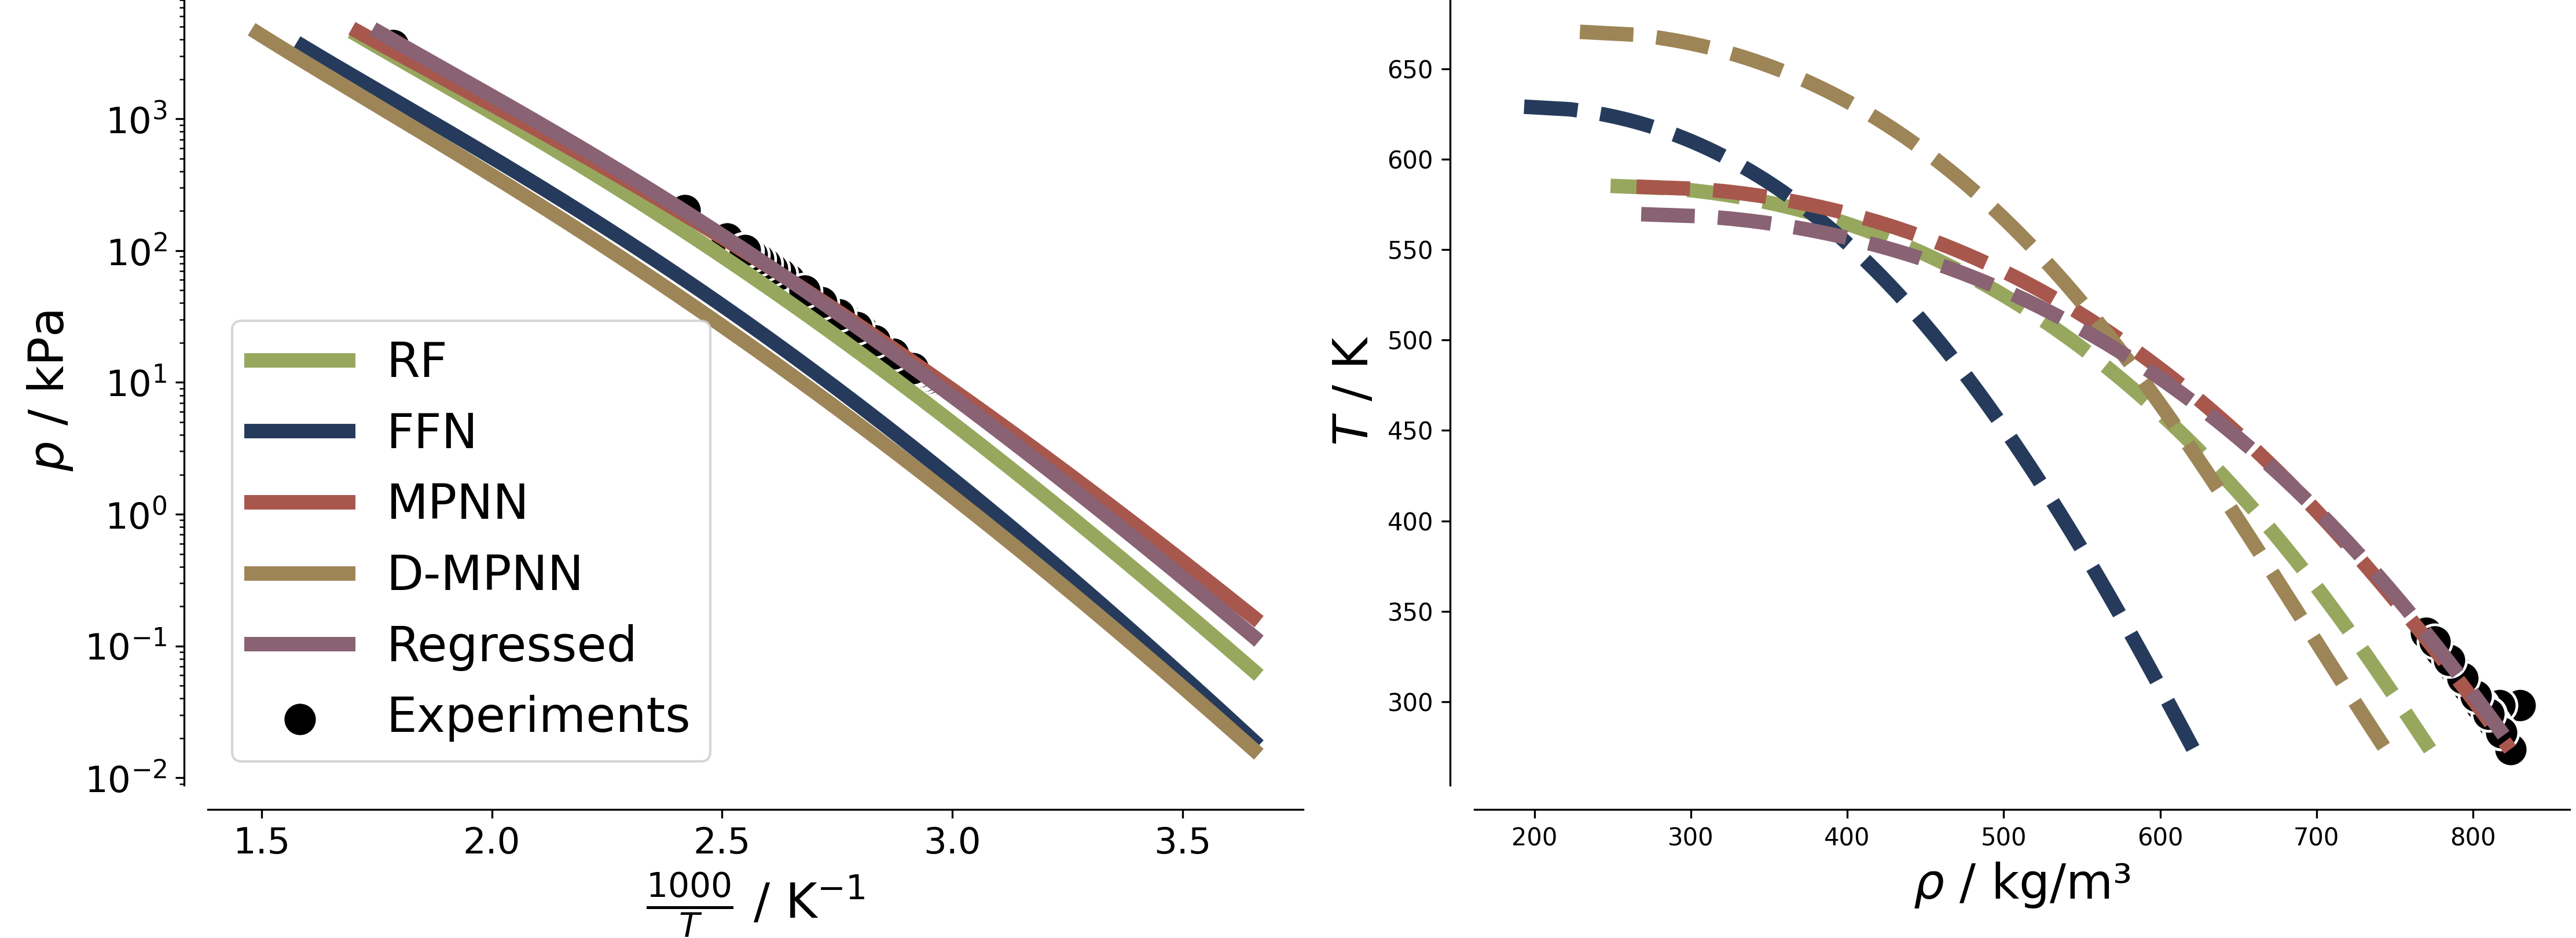
\includegraphics[width=\textwidth]{gfx/Chapter08/2-Pentanol.png}
%     \caption{Vapor pressure and density predictions of 2-pentanol of PCP-SAFT using predictions from various machine learning models}
%     \label{fig:two_pentanol}
% \end{figure}


\subsection{Comparison to existing predictive PCP-SAFT methods}

I compared ML-SAFT to predictions from the QM method SEPP \cite{Kaminski2020} and the group contribution from Sauer et al \cite{Sauer2014}.  Please note that the number of test molecules reduces to 72 as SEPP could not provide predictions to 11 molecules due to its inability to predict halogens. When comparing to SEPP, the RF produces more accurate vapor pressure predictions, while SEPP leads to more accurate density predictions, as shown in Table \ref{tab:sepp}. However, SEPP has a significant associated computational cost that can extend into days, including conformer generation, two DFT calculations, and a COSMO calculation. In contrast, ML-SAFT methods immediately predict the PCP-SAFT parameters from a SMILES string in milliseconds for each molecule while still maintaining a competitive predictive accuracy.  


\begin{table}
	\caption{Comparison of thermodynamic predictions using PCP-SAFT parameters predicted by ML-SAFT models and SEPP.\cite{Kaminski2020} The best score for each thermodynamic quantity is marked in bold. $n$ is the number of molecules in the test set that each method can predict.}
        \label{tab:sepp}
	\begin{center}
        \begin{tabular}{lrrrrr|r}
            & FFN & D-MPNN & MPNN & RF & SEPP & Regressed \\
            \hline
            $n$ & 72 & 72 & 72 & 72 & 72 & 72 \\
            \%AAD $p_{sat}$ & 372 & 49.2 & 67.8 & \textbf{39.5} & 111 & 4.51 \\
            \%AAD $\rho^{L}$ & 11.7 & 9.54 & 13.3 & 8.88 &\textbf{5.10} & 0.82 \\
            \hline
        \end{tabular}
	\end{center}
\end{table}
% Furthermore, wowe found empirically that our heuristic for identifying associating and non-associating molecules using RDKit\cite{rdkit} worked more effectively than the algorithm based on COSMO charge density used in SEPP.

Comparison with the group contribution method was impaired by the need to convert molecules to groups prior to predictions. Only 13 of the molecules in the test set had functional groups that were already parameterized in the database by Sauer et al \cite{Sauer2014}. For this small group of molecules, the RF predictions were significantly more accurate than the GC method for vapor pressure, while the D-MPNN predictions performed best for density. 


\begin{table}
	\caption{Comparison of thermodynamic predictions using PCP-SAFT parameters predicted by ML-SAFT models and a group contribution method (GC) \cite{Sauer2014}. The best score for each thermodynamic quantity  is marked in bold. $n$ is the number of molecules in the test set that each method can predict.}
    \label{tab:gc}
	\begin{center}
		\begin{tabular}{lrrrrr|r}
			 & FFN & D-MPNN & MPNN & RF & GC & Regressed \\
			\hline
			$n$ & 13 & 13 & 13 & 13 & 13 & 13 \\
			\%AAD $p_{sat}$ & 132 & 41.1 & 65.7 & \textbf{39.6} & 118 & 3.28 \\
			\%AAD $\rho^{L}$ & 13.2 & \textbf{9.98} & 15.8 & 12.2 & 10.8 & 2.98 \\
                \hline
		\end{tabular}
	\end{center}
\end{table}

\subsection{Improving MPNN predictions using transfer learning}

I hypothesized that transfer learning could be used to improve the accuracy of the MPNN predictions. As noted in the methods, I used COSMO-RS \cite{Klamt1995, Klamt2010} to generate pseudo experimental data which I the processed through the same regression and training pipeline as the Dortmund data to produce a trained MPNN. I subsequently fixed the message passing encoder of the MPNN and only trained the feedforward readout network; this model I called MPNN-TL. As shown in Figure \ref{fig:cosmo_dortmund}, a subset of the molecules (289) are in both the COSMO-RS and Dortmund databank\footnotemark, and there is non-zero correlation between the PCP-SAFT parameters regressed for several PCP-SAFT parameters. This suggests that the data regressed from COSMO-RS simulations could be a good pretraining task. 
\footnotetext{The molecules that were in both the Dortmund database and COSMO-RS database were removed from the COSMO-RS training set to prevent inflating test set performance.}

\begin{figure}
    \centering
    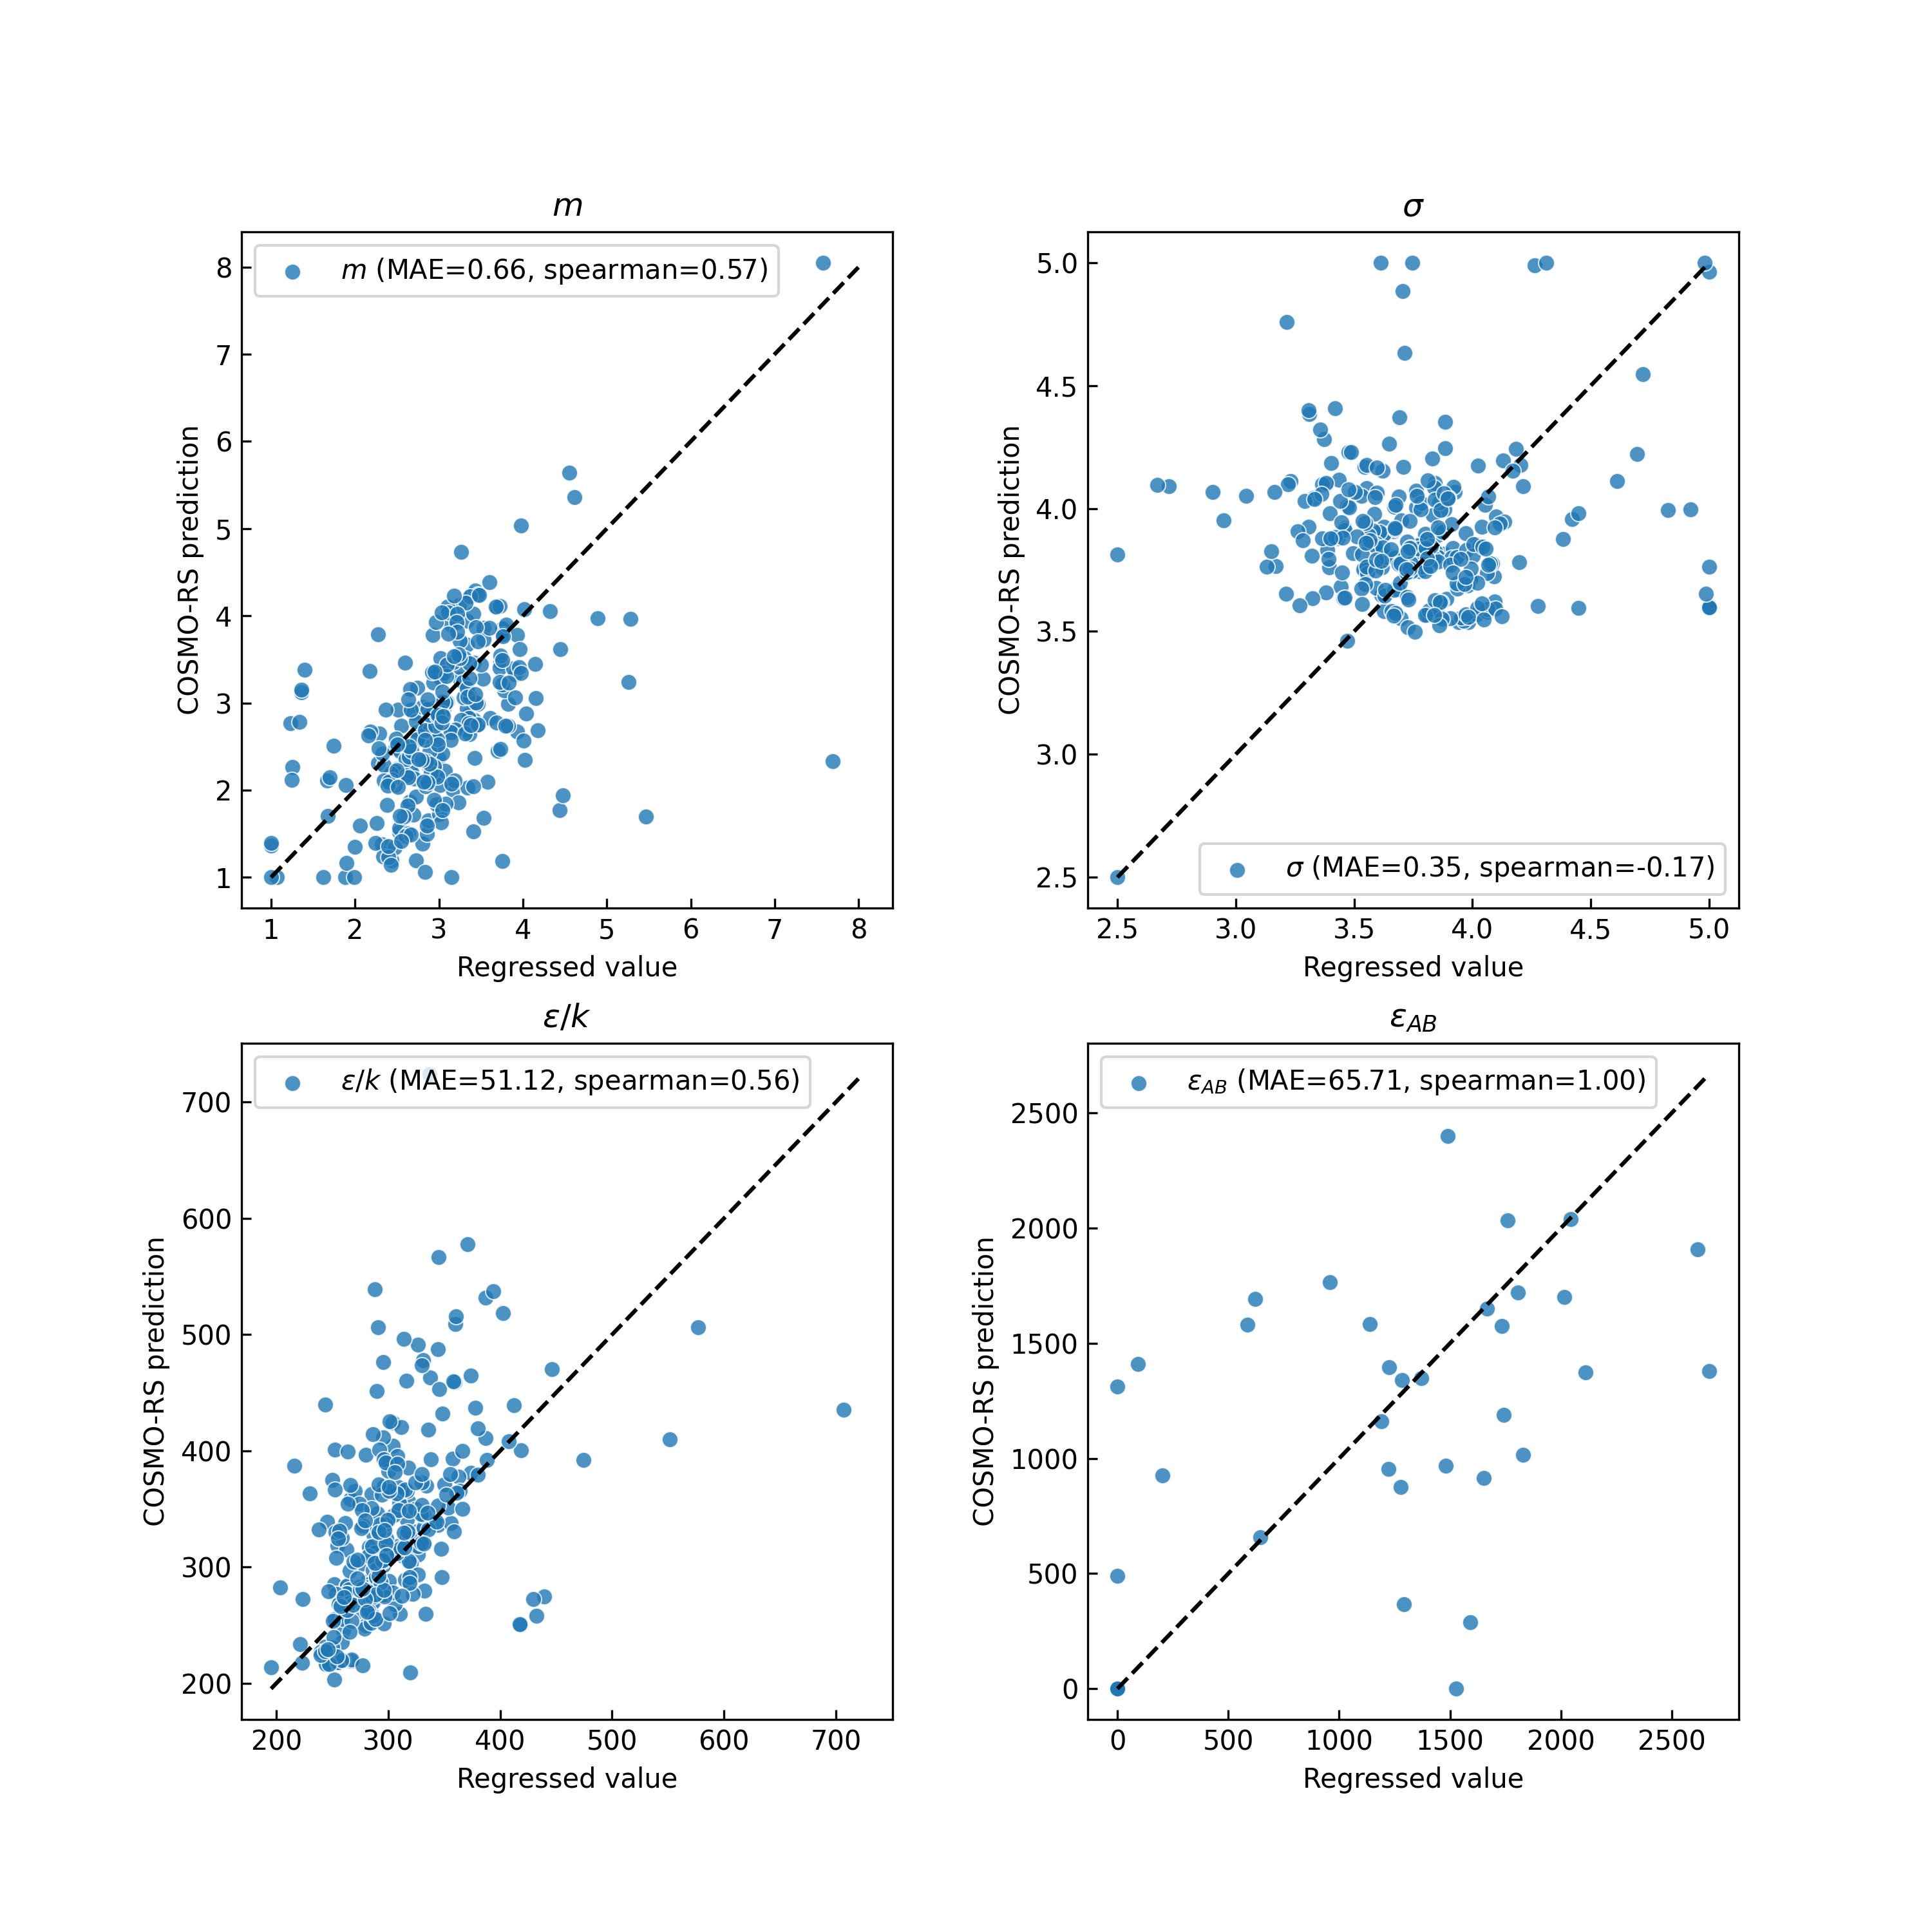
\includegraphics[width=\textwidth]{gfx/Chapter08/cosmo_dortmund_parameter_correlations.png}
    \caption{Parity plots comparing regressed PCP-SAFT parameters based on data from COSMO-RS simulations and the Dortmund databank.}
    \label{fig:cosmo_dortmund}
\end{figure}

The results of the pre-training approach are shown in Table \ref{tab:scores_tl}. On the test set, MPNN-TL outperforms the MPNN giving more accurate predictions of vapor pressure that are on par with the RF. Similarly, the MPNN makes more accurate predictions of density than both the standard MPNN and RF. These results demonstrate that using simulation data can improve the accuracy of neural networks by broadening the scope of molecule data seen during their training. 

\begin{table}
    \caption{Comparison of thermodynamic predictions using PCP-SAFT parameters predicted by MPNN model with and without transfer learning and the random forest. The best score for each thermodynamic quantity  is marked in bold. $n$ is the number of molecules in the test set that each method can predict.}
    \begin{center}
            \begin{tabular}{lrrr|r}
                & MPNN & MPNN-TL & RF & Regressed \\
                \hline
                $n$ & 81 & 81 & 81 & 81 \\
                \%AAD $p_{sat}$ & 69.73 & 50.63 & \textbf{38.55} & 4.47 \\
                \%AAD $\rho^{L}$ & 13.86 & \textbf{5.56} & 8.64 & 0.80 \\
                \hline
            \end{tabular}
    \end{center}
    \label{tab:scores_tl}
\end{table}

\section{Conclusions}

In this chapter, I proposed ML-SAFT, a machine learning framework for prediction of PCP-SAFT parameters directly from molecular structures. I developed the largest database of PCP-SAFT parameters (988 molecules) derived from the Dortmund databank. ML-SAFT trained on this dataset accurately predicted the regressed PCP-SAFT parameters, and these predicted PCP-SAFT parameters could be in turn used for accurate predictions of thermodynamic quantities. Random forests had the highest accuracy for the regressed PCP-SAFT parameters and the thermodynamic predictions overall.

The best ML-SAFT model (random forests) performed comparably with or better than existing predictive PCP-SAFT methods while being applicable to a wider range of molecules and giving fast predictions. Group contribution methods require new molecules to be fragmented into groups, and I found that a large fraction of molecules in the dataset were missing parameterized groups or could not be resolved by the automatic fragmentation algorithm. On the other hand, the QM method used for comparison, SEPP, currently is restricted to molecules without halogens as the linear regression model was only fit on alkanes. Furthermore, SEPP requires significant computational time for each molecule, while ML-SAFT affords accurate predictions on a wide range of molecules in milliseconds. Note that even though random forests performed best, they are known for having poor extrapolation capabilities. Therefore, I expect that the models will not extend to compound classes not included in the training dataset.

Furthermore, I demonstrated that transfer learning from COSMO-RS simulations to experimental data improved the performance of deep learning models. This result reflects previous literature that shows that pretraining with simulation data for the same task can augment performance of message passing neural networks \cite{Vermeire2021}. In contrast to chapter \ref{ch:deep_gamma}, the pretraining and primary tasks were the  same. This suggests that one essential part of transfer learning using message passing neural networks is matching the pretraining and primary tasks. Future work could construct hand-designed source (pretraining) and targets task sets with different underlying distributions to further investigate what causes transfer learning to fail.

There are several ways in which ML-SAFT could be improved. First, the training data for ML-SAFT was primarily small molecules with less than 15 atoms. Previous work has shown that PCP-SAFT can effectively predict properties of larger drug-like molecules (e.g., solubility) \cite{Klajmon2020}, and the success of MPNNs in predicting the properties of drug-like molecules suggests that ML-SAFT would be effective given sufficient training data. Seconds, large fraction of the Dortmund dataset was not used because there was not high quality vapor pressure and density data for a large fraction of the molecules (a requirement for PCP-SAFT parameter regression). Future work could explore how to integrate the PCP-SAFT equation into the training of neural networks so that the model could be trained end-to-end to predict vapor pressure and density. Since neural networks are trained via batch gradient descent, it would be possible to use the datasets for which there are not both vapor pressure and density data. Third, I do not predict the binary interaction coefficients, which has been shown to significantly improve the quality of PCP-SAFT predictions for mixtures. Future work could address this limitation by training models that contain message-passing between two molecular graphs. This would be a next step towards accurate predictions of multi-component mixture properties using PCP-SAFT.


